\everymath{\displaystyle}
\documentclass{beamer}
% \documentclass[handout]{beamer}

%\usepackage[pdftex]{color,graphicx}
\usepackage{amsmath,amssymb,amsfonts}

\mode<presentation>
{
  % \usetheme{Darmstadt}
  % \usetheme[hideothersubsections]{Hannover}
  % \usetheme[hideothersubsections]{Goettingen}
  \usetheme[hideothersubsections, right]{Berkeley}

  \usecolortheme{seahorse}
  % \usecolortheme{dolphin}
  \usecolortheme{rose}
  % \usecolortheme{orchid}

  \useinnertheme[shadow]{rounded}

  % \setbeamercovered{transparent}
  \setbeamercovered{invisible}
  % or whatever (possibly just delete it)
}

\mode<handout>{
  \setbeamercolor{background canvas}{bg=black!5}
  \usepackage{pgfpages}
  \pgfpagesuselayout{4 on 1}[a4paper,border shrink=5mm, landscape]
}

\usepackage[brazilian]{babel}
% or whatever

% \usepackage[latin1]{inputenc}
\usepackage[utf8]{inputenc}
% or whatever

\usepackage{times}
%\usepackage[T1]{fontenc}
% Or whatever. Note that the encoding and the font should match. If T1
% does not look nice, try deleting the line with the fontenc.


\title[Seminário] % (optional, use only with long paper titles)
{Seminário de artigo}

\subtitle
{Análise Pré e Pós-Operatória da Capacidade Funcional e Qualidade de Vida de Pacientes Portadores de Osteoartrose de Quadril Submetidos à Artroplastia Total} % (optional)

\author%[] % (optional, use only with lots of authors)
{Felipe Figueiredo}% \and S.~Another\inst{2}}
% - Use the \inst{?} command only if the authors have different
%   affiliation.

\institute[INTO] % (optional, but mostly needed)
{Mestrado Profissional em Ciências Aplicadas ao Sistema Musculoesquelético\\
Instituto Nacional de Traumatologia e Ortopedia Jamil Haddad
}
  % \inst{1}%
  % Department of Computer Science\\
  % University of Somewhere
  % \and
  % \inst{2}%
  % Department of Theoretical Philosophy\\
  % University of Elsewhere}
% - Use the \inst command only if there are several affiliations.
% - Keep it simple, no one is interested in your street address.

\date%[] % (optional)
{07/12/2017}

% \subject{Talks}
% This is only inserted into the PDF information catalog. Can be left
% out. 



% If you have a file called "university-logo-filename.xxx", where xxx
% is a graphic format that can be processed by latex or pdflatex,
% resp., then you can add a logo as follows:

\pgfdeclareimage[height=1.6cm]{university-logo}{logo}
\logo{\pgfuseimage{university-logo}}



% Delete this, if you do not want the table of contents to pop up at
% the beginning of each subsection:
\AtBeginSubsection[]
%\AtBeginSection[]
{
  \begin{frame}<beamer>{Sumário}
    \tableofcontents[currentsection,currentsubsection]
  \end{frame}
}


% If you wish to uncover everything in a step-wise fashion, uncomment
% the following command: 

% \beamerdefaultoverlayspecification{<+->}


\begin{document}

\begin{frame}
  \titlepage
\end{frame}

% \begin{frame}{Sumário}
%   \tableofcontents
%   % You might wish to add the option [pausesections]
% \end{frame}


%% Template
% \section{}

% \subsection{}

% \begin{frame}{}
%   \begin{itemize}
%   \item 
%   \end{itemize}
% \end{frame}

% \begin{frame}
%   \begin{columns}
%     \begin{column}{5cm}
%     \end{column}
%     \begin{column}{5cm}
%     \end{column}
%   \end{columns}
% \end{frame}

% \begin{frame}{}
%   \includegraphics[height=0.4\textheight]{file1}
%   \includegraphics[height=0.4\textheight]{file2}
%   \includegraphics[height=0.4\textheight]{file3}
%   \begin{figure}
%     \caption{}
%   \end{figure}
% \end{frame}

% \begin{frame}{}
%   \begin{definition}
%   \end{definition}
%   \begin{example}
%   \end{example}
%   \begin{block}{Exercício}
%   \end{block}
% \end{frame}

\section{Artigo}

\subsection{Intro}

\begin{frame}{}
  \begin{center}
    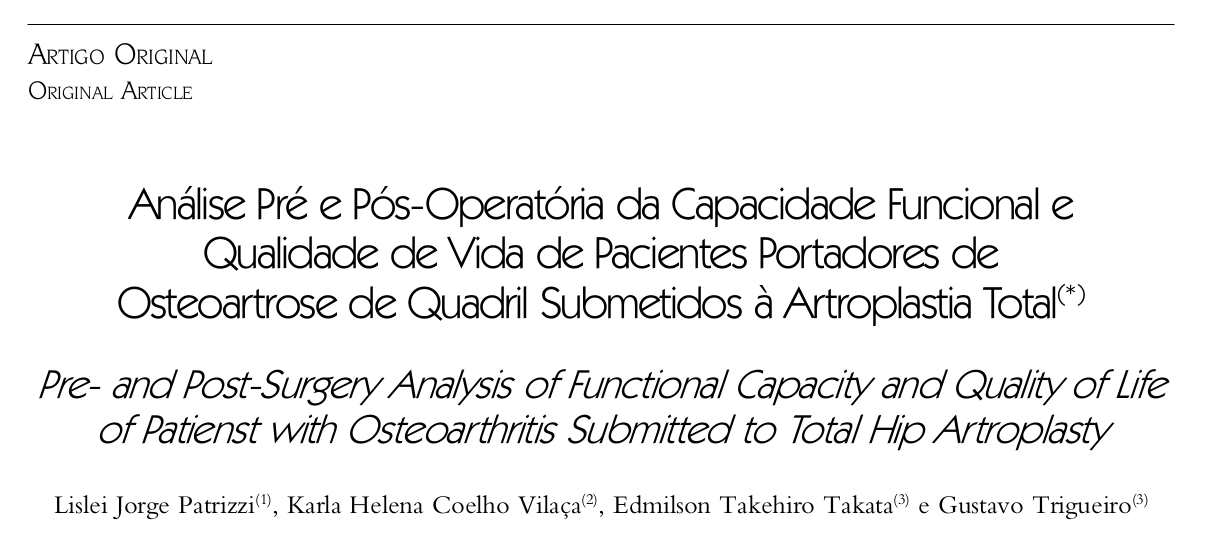
\includegraphics[width=.9\textwidth]{figuras/titulo}
  \end{center}
\end{frame}

\begin{frame}{}
  \begin{center}
    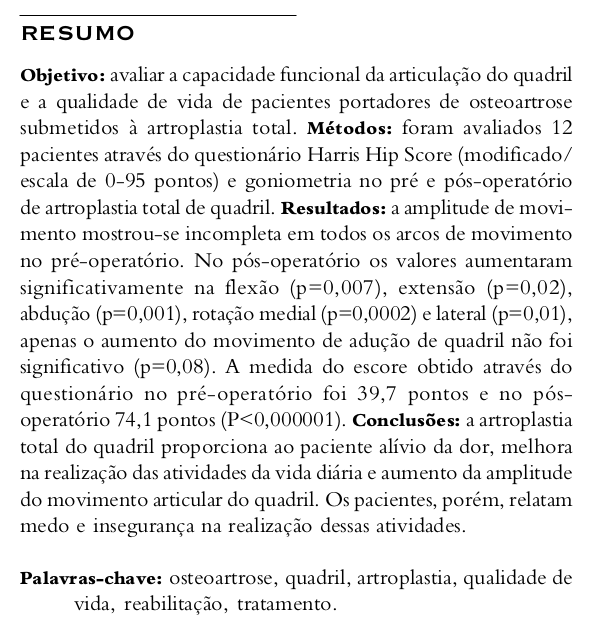
\includegraphics[height=.9\textheight]{figuras/resumo}
  \end{center}
\end{frame}

\subsection{Métodos}

\begin{frame}{}
  \begin{center}
    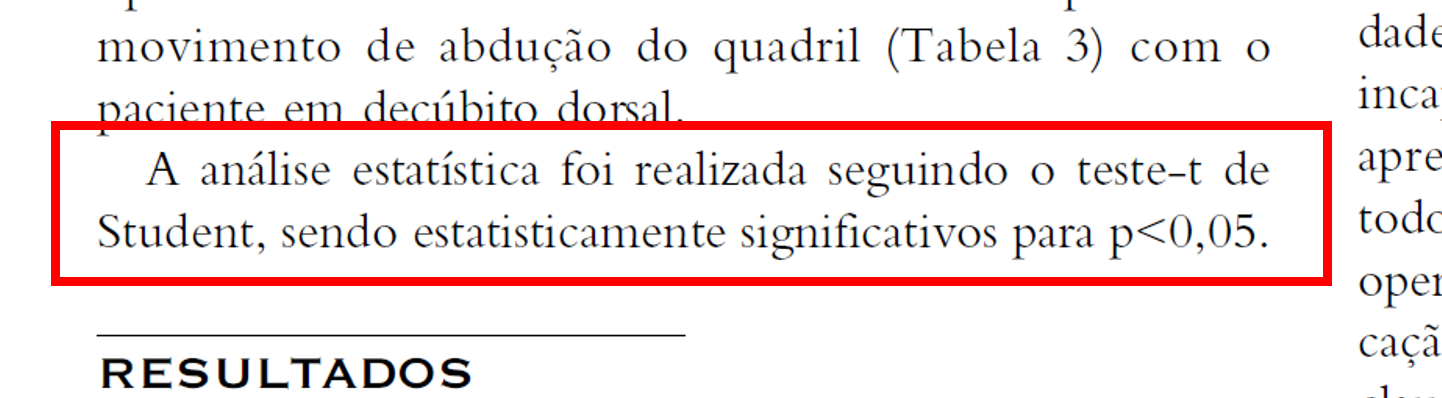
\includegraphics[width=\textwidth]{figuras/metodologia}
  \end{center}
\end{frame}

\begin{frame}{Dados brutos (N=12)}
  \begin{center}
    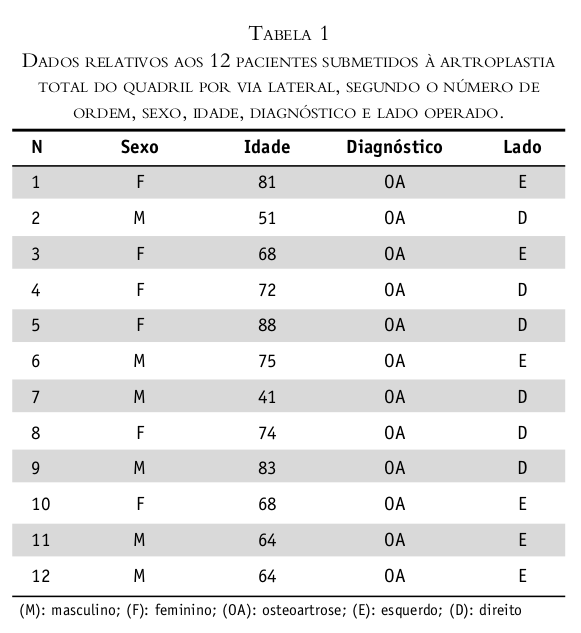
\includegraphics[height=.9\textheight]{figuras/tabela1}
  \end{center}
\end{frame}

\begin{frame}{Métodos}
  \begin{itemize}
  \item Questionário Harris Hip Score - HHS (0-100)
  \item Alteração: amplitude de movimento mensurado à parte (HHS; 0-95)
  \item Mensuração da amplitude de movimento em goniômetro
  \end{itemize}
\end{frame}

\begin{frame}{Questionário Harris Hip Score}
  \begin{center}
    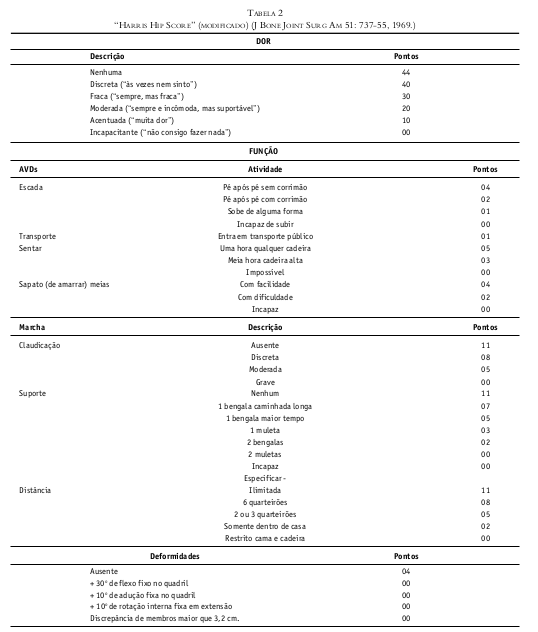
\includegraphics[height=.9\textheight]{figuras/tabela2}
  \end{center}
\end{frame}

\begin{frame}{Goniometria}
  \begin{center}
    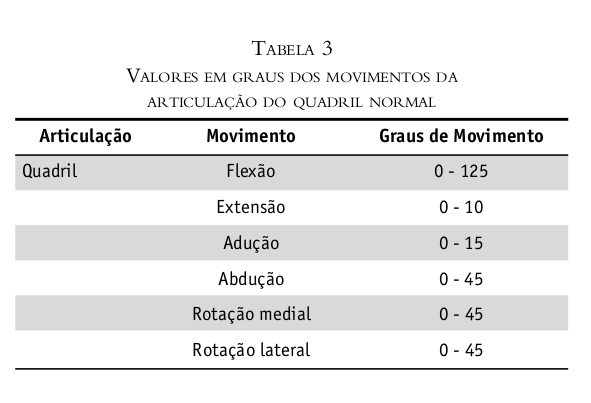
\includegraphics[height=.9\textheight]{figuras/tabela3}
  \end{center}
\end{frame}

\subsection{Análise Descritiva}

\begin{frame}{Análise Descritiva}
  \begin{itemize}
  \item pré-operatório: média = 39,7 pontos, mediana = 35,00, desvio
padrão = 11,8  {\em ``desvio padrão com relação à média de''} 3,4
\item pós-operatório: média = 74,2 pontos, mediana = 74,00, desvio padrão = 11,2
e {\em ``um desvio padrão com relação à média de''} 3,2.
\item {\em ``intervalo de confiança com 95\% de significância''} para a diferença entre pares: de -44,27 a -24,73
  \end{itemize}
\end{frame}

\begin{frame}{}
  \begin{center}
    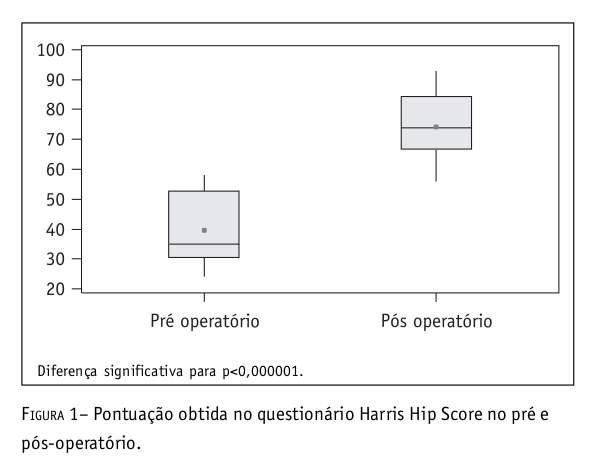
\includegraphics[height=.9\textheight]{figuras/figura1}
  \end{center}
\end{frame}

\subsection{Testes}

\begin{frame}{}
  \begin{center}
    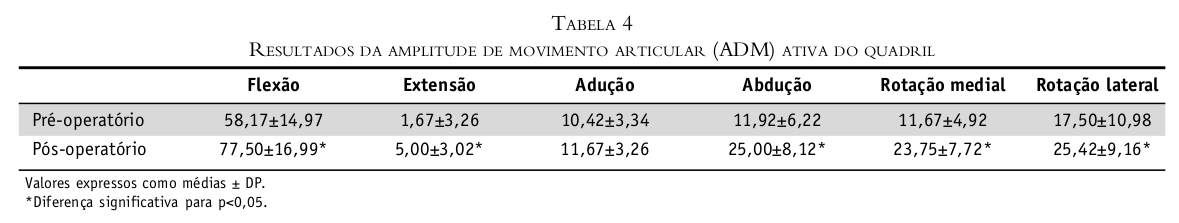
\includegraphics[width=1.15\textwidth]{figuras/tabela4}
  \end{center}
\end{frame}

\subsection{Conclusões}

\begin{frame}{Conclusões}
  \begin{block}{}
    Conclui-se que a artroplastia total do quadril devolve aos pacientes portadores de osteoartrose uma amplitude de movimento articular próxima da normalidade, aliviando a dor e facilitando a realização das atividades da vida diária.
    No entanto, esses pacientes referiram medo e insegurança na realização dessas atividades.
  \end{block}
\end{frame}

\section{Avaliação crítica}

\subsection{Avaliação crítica}

\begin{frame}{Problemas observados}
  \begin{center}
    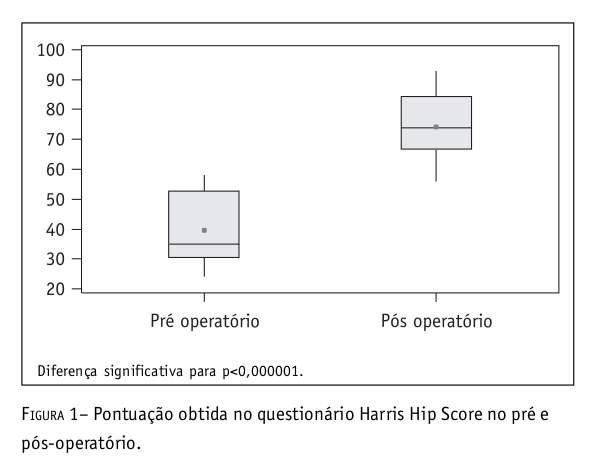
\includegraphics[height=.5\textheight]{figuras/figura1}
  \end{center}
  \begin{block}{Hipótese}
    A figura 1 indica que talvez os autores tenham utilizado o teste t para grupos independentes.
  \end{block}
\end{frame}

\begin{frame}{Problemas observados}
  \begin{center}
    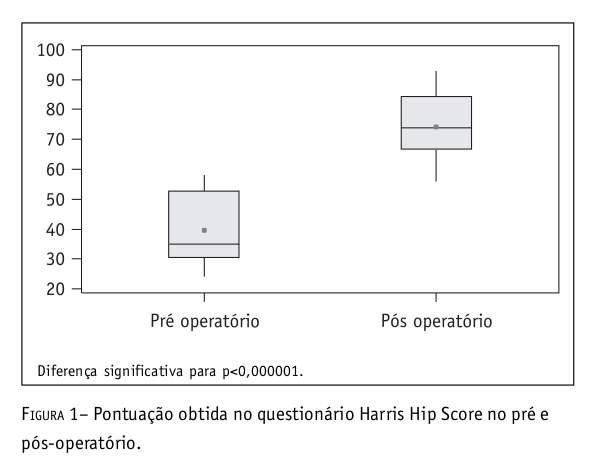
\includegraphics[height=.5\textheight]{figuras/figura1}
  \end{center}
  \begin{itemize}
  \item Os grupos são pareados (pré e pós operatório)
  \item O teste adequado seria o teste t para grupos dependentes/pareados
  \item Os valores da tabela 4 podem ser usados para conferir esta hipótese
  \end{itemize}
\end{frame}

\begin{frame}{Reproduzindo}
  \begin{center}
    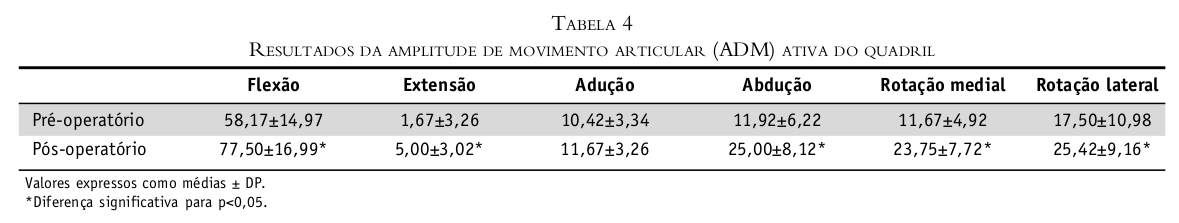
\includegraphics[width=1.15\textwidth]{figuras/tabela4}
  \end{center}
  \begin{exampleblock}{Extensão}
    \begin{itemize}
    \item pré: $1.67 \pm 3.26$
    \item pós: $5.00 \pm 3.02$
    \item p-valor declarado no texto: $p=0.02$
    \end{itemize}
  \end{exampleblock}
\end{frame}

\begin{frame}{(após uma breve busca no Google)}
  \begin{center}
    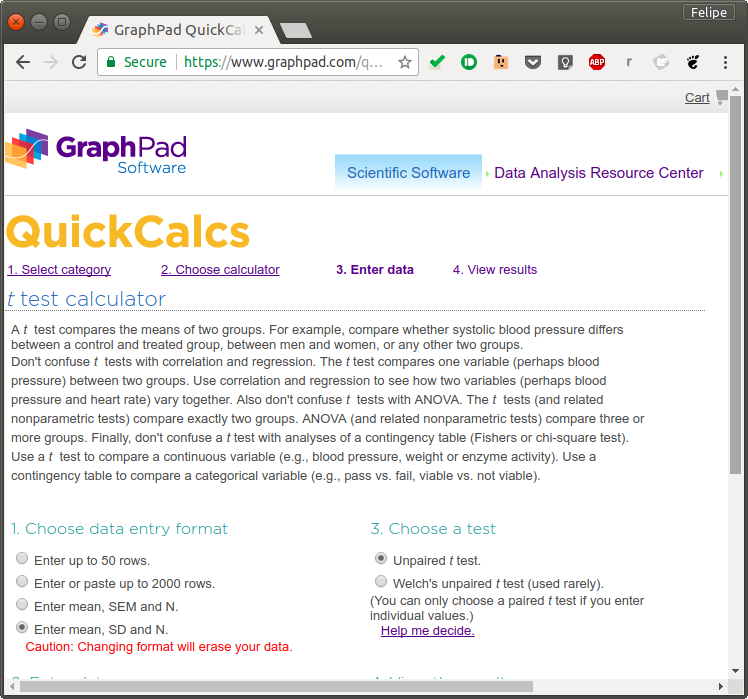
\includegraphics[height=.9\textheight]{figuras/teste-t1}
  \end{center}  
\end{frame}

\begin{frame}{Reproduzindo}
  \begin{center}
    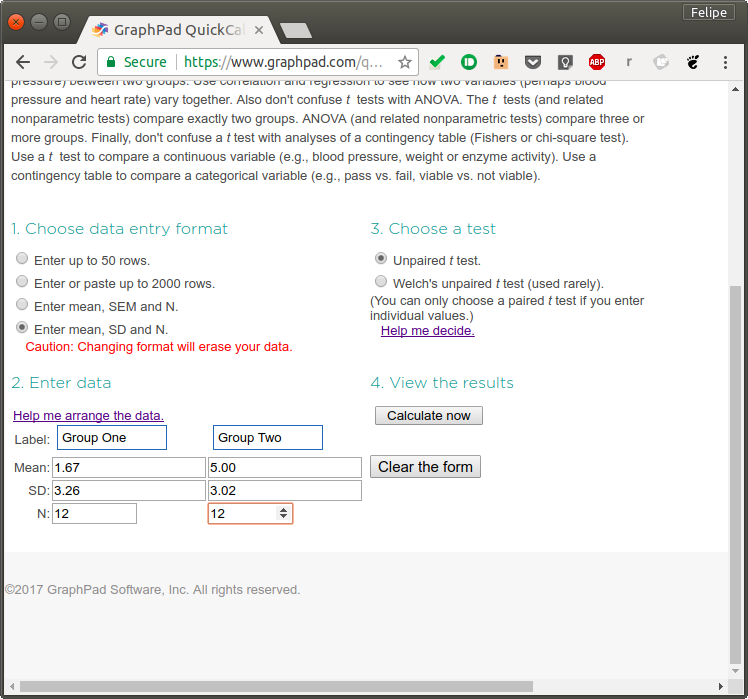
\includegraphics[height=.9\textheight]{figuras/teste-t2}
  \end{center}  
\end{frame}

\begin{frame}{Reproduzindo}
  \begin{center}
    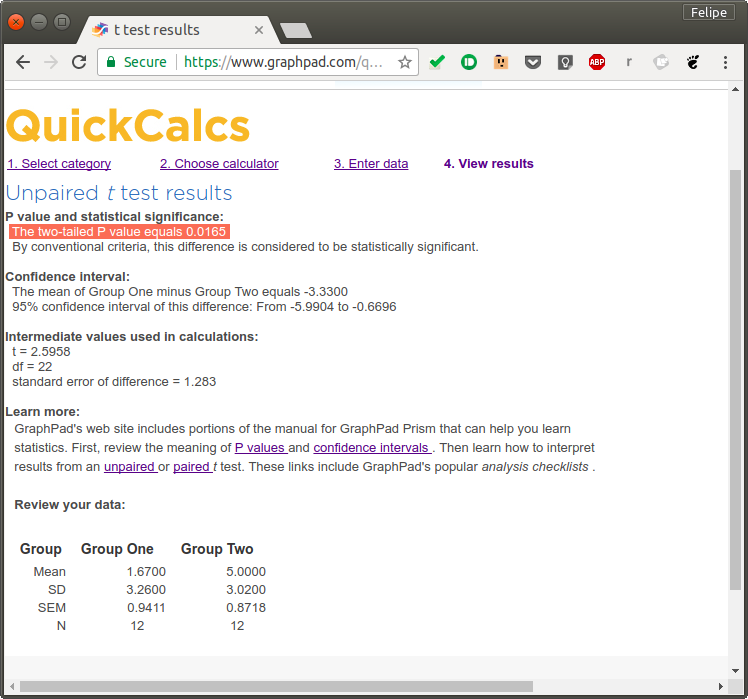
\includegraphics[height=.9\textheight]{figuras/teste-t3}
  \end{center}  
\end{frame}

\begin{frame}{Conclusão}
  \begin{itemize}
  \item O teste utilizado para a comparação pré e pós operatória foi o teste t para grupos independentes
  \item Outras comparações do artigo usaram o mesmo teste (resultados não mostrados)
  \item Este é um erro metodológico, já que os grupos são dependentes
  \end{itemize}
\end{frame}

% \begin{frame}{Conclusões não retornam às hipóteses}
%   % \begin{center}
%   %   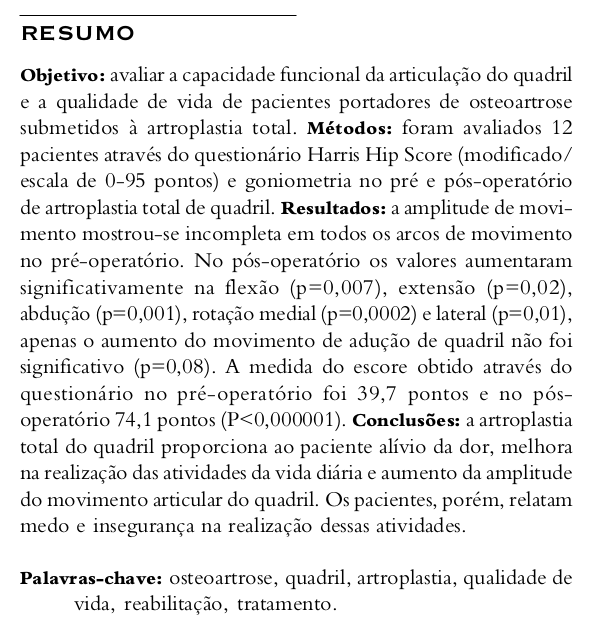
\includegraphics[height=.5\textheight]{figuras/resumo}
%   % \end{center}
%   \begin{block}{}
%     {\bf Objetivo:} avaliar a capacidade funcional da articulação do quadril e a qualidade de vida de pacientes portadores de osteoartrose submetidos à artroplastia total.

%     \bigskip
%     {\bf Métodos:} questionário Harris Hip Score e goniometria no pré e pós-operatório de artroplastia total de quadril.

%     \bigskip
%     {\bf Conclusões:} a artroplastia total do quadril proporciona ao paciente alívio da dor, melhora na realização das atividades da vida diária e aumento da amplitude do movimento articular do quadril. Os pacientes, porém, relatam medo e insegurança na realização dessas atividades.
%   \end{block}
% \end{frame}

\begin{frame}{Problemas observados (2)}
  \begin{itemize}
  \item Os dados são {\bf escores} (de 0 a 95)
  \item Não há nenhuma razão para {\em acreditar} que sejam normalmente distribuídos
  \item Os autores não fizeram um teste contra normalidade
  \item Por construção, um teste não-paramétrico é mais apropriado (Wilcoxon)
  \end{itemize}
\end{frame}

\end{document}
